\chapter{Implementation}

\section{Tools \& Technologies}

\subsection{Node.js}
I decided early on that this application should be easily accessible on a range of devices, particularly the game interface. For this reason I built the system as a responsive web-application, running on a node server. Node\cite{Node} is an excellent framework for getting sizeable projects up and running very quickly, which I was able to do with this project. This is in part due to NPM\cite{npm}, which provides access to countless packages which I was able to use, ranging from Victory\cite{Victory} for visualisations, to Thunk\cite{Thunk} for managing asynchronous side effects.

\subsection{TypeScript}
According to Microsoft who maintain it, `TypeScript is a typed superset of JavaScript that compiles to plain JavaScript'\cite{Typescript}. 
I decided to use TypeScript (TS) to combat some of the problems that can occur when working on a large JavaScript codebase. 
Being statically typed, TS prevents type errors and instantly makes code more navigable and readable. 
This helps both during development and maintenance, which is particularly important if others continue to work on this project.

\subsubsection{React}
React\cite{React} is a UI library that simplifies the creation of responsive interface components. I knew that I wanted my application to be highly responsive, with each section effectively being split into a single page application. React made this fairly trivial once the structure of the page was settled, as information flows down through components and they are automatically updated.

\subsubsection{Redux}
Redux\cite{Redux} complements React nicely, by helping to manage state. When using pure React, each component stores it's own state. This can make things confusing as components that should be reflecting information can fall out of sync. Redux encourages moving the state of the whole application into one top-level serializable JS object. This then acts aas a `single source of truth', which takes care of several considerations. Another benefit that I found redux to have is the debugging tools, which take the form of a chrome extension\cite{ReduxDev}. When Redux is correctly used, this tool makes it possible to view and manipulate the application state, and even `time travel' the page to a previous state, such as before a button was clicked. This made debugging very straightforward, particularly for the game logic.

\begin{figure}[!h]
	\centering
	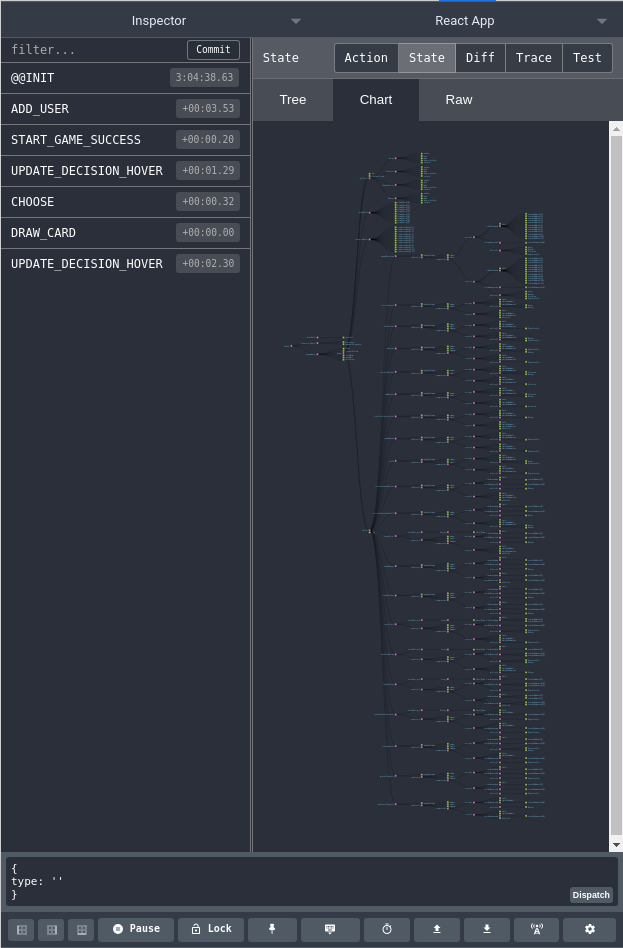
\includegraphics[width=0.8\textwidth]{./images/impl/redux_view.png}
	\caption{Redux DevTool\cite{ReduxDev} opened in game view. This shows what actions have occurred while the page has been open, as well as visualising the application state.}
	\label{fig:redux_view}
\end{figure}

\subsection{NeDB}
To store both the game definitions and the gameplay data, I needed a form of server-side persistance. I had to decide here between designing and maintaining a rigid relational database, or opting for a NoSQL\cite{NoSQL} solution. After consideration, I chose to go with a document-based database. The main factor in this decision was that I was unsure of what data would be desired by users of the final product. While a relational database requires strict definitions of data and their types, document-based databases are much more free form, meaning values can be added and removed with no alterations to the database server required.

Specifically, I chose to use NeDB\cite{NeDB}. NeDB is a lightweight JS database library that was quick and easy to set up and use. The API it provides is a subset of that of MongoDB\cite{MongoDB}, and was therefore well documented despite this being a smaller, more lightweight tool. Game definitions and user data are stored in two separate instances.

This database implementation does have some downsides in terms of long term maintenance - ideally further along in the project's life cycle this would probably be converted to a relational database, once the data requirements were more strictly defined. Also, regrettably NeDB does not expose encryption as part of its API.
This was something I only became aware of towards the end of the project, I might have chosen a different library if this had been immediately obvious. It would still be possible to encrypt fields individually
It did however suit the needs of the project, and I believe I made the right choice in getting started with NoSQL.

\section{Frontend}

